%%%%%%%%%%%%%%%%%%%%%%%%%%%%%%%%%%%%%%%%%%%%%%%%%%%%%%%%%%
%
% Doctoral Thesis Template @ The University of Manchester
% LaTeX Chapter Template
% Version 1 (23/07/2020)
% Joe Crone
%
% This template is based on:
% The University of Manchester, Presentation of Thesis Policy
% Research Office Graduate Education Team
% June 2017
% http://www.regulations.manchester.ac.uk/pgr-presentation-theses/
%
%%%%%%%%%%%%%%%%%%%%%%%%%%%%%%%%%%%%%%%%%%%%%%%%%%%%%%%%%%
\documentclass[../main.tex]{subfiles}
\begin{document}

% Title
%--------------------------------------------------------
\chapter{CBETA Multi-Turn Commissioning}
\label{CBETA_Multi-Pass_Commissioning} % to reference use \ref{ChapterTemplate}

\section{Energy Recovery Linacs}

\section{Multi-Turn ERLs}

\section{CBETA Commissioning}
% CBETA motivation, USP + context
\subsection{CBETA Motivation and Context}

The Cornell University (CU) Brookhaven National Laboratory (BNL) Energy Recovery Linac Test Accelerator (CBETA) is a 4-turn superconducting RF ERL test facility, which utilises a novel non-scaling FFA (ns-FFA) return loop for re-circulation and energy recovery of electron bunches \cite{hoffstaetter2017cbeta,bartnik2020cbeta}. The 4-turn (8-pass) ERL was built in collaboration with BNL and hosted at Cornell University -- the birthplace of the ERL concept \cite{tigner1965possible}. A schematic of the CBETA ERL is shown in Fig.~\ref{fig:CBETA_Layout}

\begin{figure}[!h]
\centering
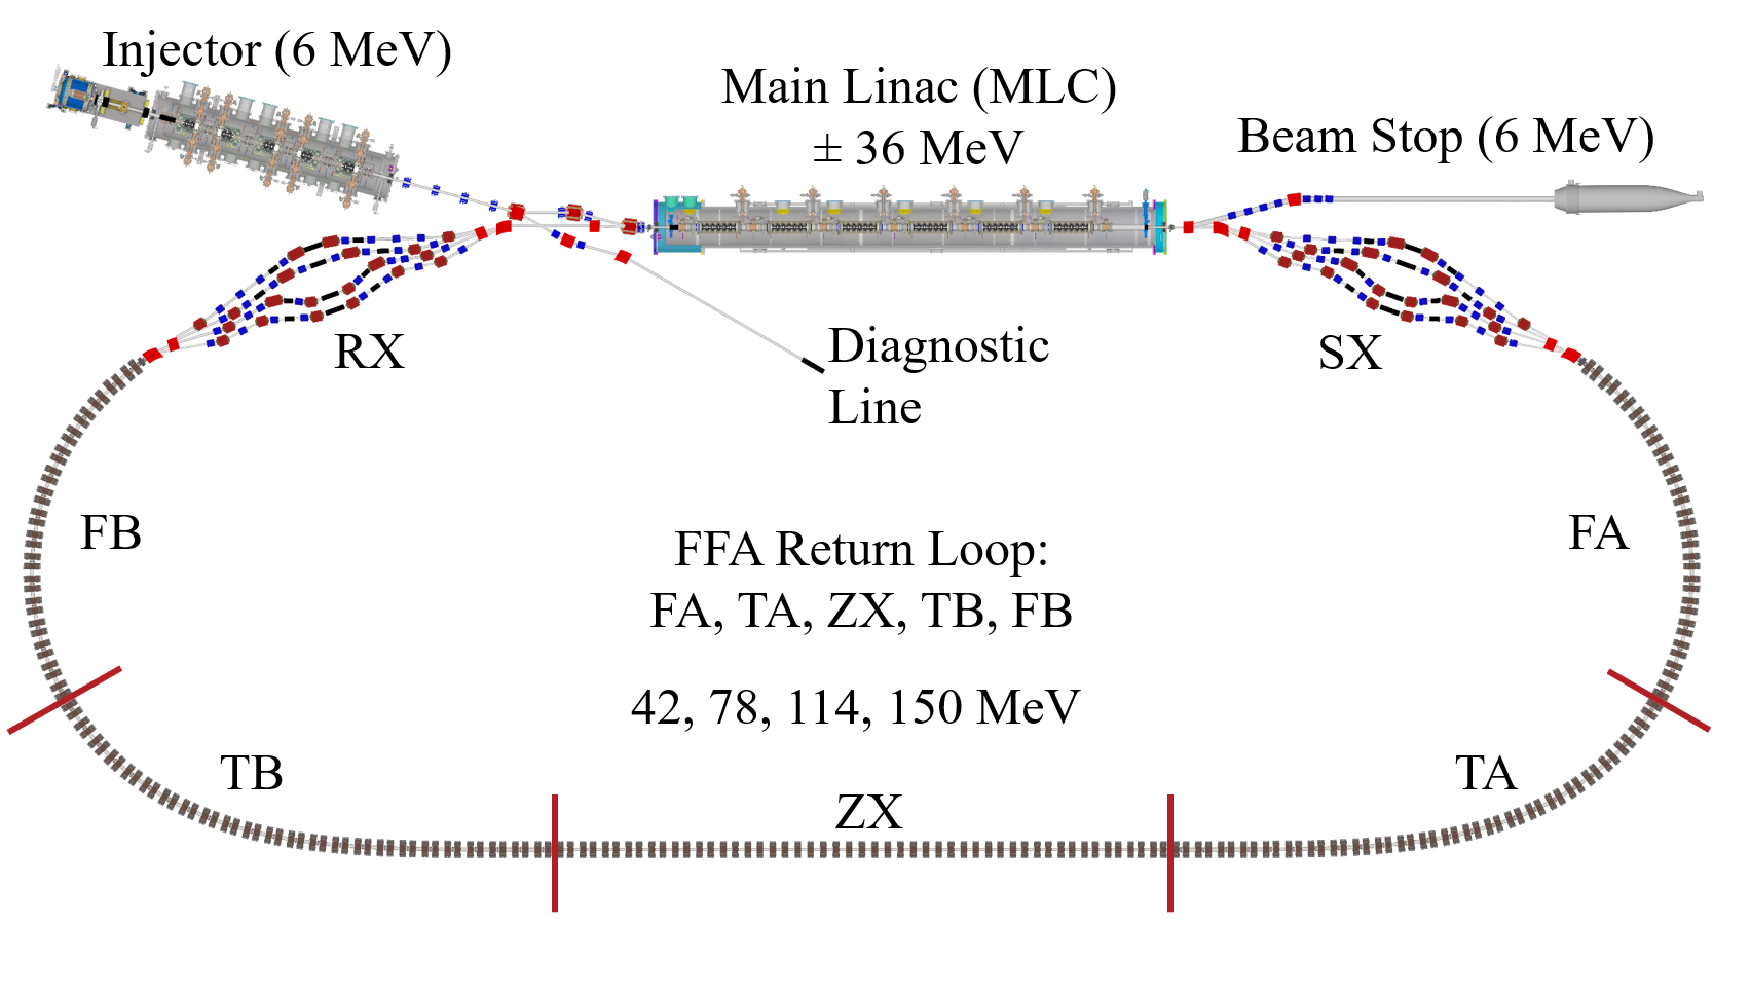
\includegraphics[width=0.8\textwidth]{Figures/CBETA_Multi-Pass_Commissioning/CBETA_4turn.pdf}
\caption{Schematic of the CBETA ERL. The electron bunch is produced by the photo-injector ($E_{\mathrm{inj}} = 6$~\si{\mega\electronvolt}), accelerated by the main linac ($\Delta E_{e} = \pm 36$~\si{\mega\electronvolt}) and re-circulated by the FFA return loop (FA--FB) for 4 successive passes until the maximum electron energy is reached ($E_{e} = 150$~\si{\mega\electronvolt}). The designed path length induces a phase change of 180\si{\degree} on the 5th pass such that the electron beam is decelerated for the next 4 passes, where the electron bunch is returned to the injection energy on the 8th pass and transported to the beam stop.}
\label{fig:CBETA_layout}
\end{figure}

The CBETA ERL was originally envisioned as a test-bed of the ERL approach to a coherent electron cooler \cite{derbenev1991coherent,litvinenko2009coherent} required to improve the luminosity of the forthcoming electron--ion collider (EIC) \cite{willeke2021electron}. The multi-turn ERL concept is a favoured approach for coherent electron cooling because high brightness electron bunches of moderate kinetic energy ($E_{e} = 149.8$~\si{\mega\electronvolt} \cite{willeke2021electron}) may be delivered in a compact footprint; CBETA has a circumference of 79.1~\si{\meter}. 

An ERL driven free electron laser \cite{bazarov2003lattice,gruner2001study,bilderback2006status} was originally proposed at Cornell University to provide a hard x-ray facility, expanding the energy range of the existing CHESS synchrotron radiation facility \cite{batterman1979chess,CHESSstructuralmaterialsbeamline}. The Cornell ERL light source design consists of a 5~\si{\giga\electonvolt} single turn ERL with an average electron beam current of 100~\si{\milli\ampere} \cite{bazarov2003lattice,gruner2001study,bilderback2006status}, driving a 25~\si{\meter} free electron laser for the production of $\lambda = 6$~\si{\pico\meter} ($E_{\gamma} = 207.2$~\si{\kilo\electronvolt}) at high x-ray brilliance $\mathcal{B}_{\mathrm{avg}}\sim 10^{23}$~ph/\si{\second}~\si{\milli\meter}$^{2}$--\si{\milli\radian}$^{2}$ 0.1\% bw \cite{bilderback2006status}. Whilst the CBETA ERL is much smaller scale and energy than the Cornell ERL light source, the high electron brightness, moderate energy from the compact CBETA accelerator is advantageous toward alight source. Hence, the CBETA ERL is suggested as a electron beam driver of a hard x-ray ($E_{\gamma} = 402.5$~\si{\kilo\electronvolt}) inverse Compton scattering source in Chapter~\ref{CBETA_Inverse_Compton_Scattering_Source_Design}, providing a high energy extension to the CHESS SR facility.

\subsection{The CBETA ERL}
% how does CBETA work + why is it special

In the CBETA ERL the electron bunch is injected from a high repetition rate continuous wave photoinjector, capable of delivering high brightness electron bunches with small transverse emittance ($\epsilon_{n} = 0.3$~\si{\milli\meter}--\si{\milli\radian}) at an electron energy of 6~\si{\mega\electronvolt}. Electron bunches are produced at 325~\si{\mega\hertz} repetition rate, with the photoinjector providing an electron beam current as high as 75~\si{\milli\ampere}. The Cornell DC photo-emission gun and injector cryomodule is world-leading in both small emittance and average beam current; ideal for a high brightness ERL. The electron bunch is then accelerated by the superconducting RF main linac cryomodule (MLC), which accelerates the electron bunch to 42~\si{\mega\electronvolt} kinetic energy -- an energy gain of $\pm 36$~\si{\mega\electronvolt} per pass. The MLC is 9.8~\si{\meter} long and comprised of six 7-cell 1.3~\si{\giga\hertz} superconducting cavities providing an accelerating field of up to 16~\si{\mega\volt}/\si{\meter} \cite{hoffstaetter2017cbeta}.

Post-acceleration the electron bunch is then re-circulated via the non-scaling FFA return loop, as shown in the schematic of the CBETA ERL in Fig.~\ref{fig:CBETA_ICS_Layout}. The non-scaling FFA optics scheme is explained in Section~\ref{sec:FFA}, and in CBETA the ns-FFA return loop is used to transport the multiple energy electron beams (42, 78, 114, 150~\si{\mega\electronvolt}) using a series of Hallbach permanent magnet quadrupoles. The arcs of the ns-FFA return loop contain a periodic combined function--defocusing quadrupole doublet (FA/FB), the straight is comprised of a focusing--defocusing quadrupole doublet (ZX) and the transition sections (TA/TB) are comprised of quadrupole doublets which are offset from the reference orbit to slowly conform the electron bunch in the arcs to the reference trajectory in the straight sections (TA) and the reverse (TB) for straight to arc transition. Further information on design of the complex transition sections is presented by Hoffstaetter et al \cite{hoffstaetter2017cbeta}.  

The splitter (SX) and recombiner (RX) spreader sections merge the linac with the FFA return loop via a common transport arrangement -- both accelerating and decelerating electron beams traverse the same spreader beamline -- however, each energy has a dedicated beamline (S1--4, R1--4). The spreader sections consist of a series of linear electromagnets (quadrupoles and dipoles) and a set of bellows which adjust the path length of each turn, consequently varying the time-of-flight of the electron beam, for fine adjustment in the phase witnessed by the electron bunch upon arrival in the MLC. Adjustment of the MLC arrival phase is required for acceleration or deceleration of the electron bunch as explained in Section~\ref{sec:ERL_theory}. Since permanent magnets are used for the return loop, and electromagnets for the spreaders, the spreaders must also be used for any electron beam orbit correction.

% multi-turn + decelerations
Upon arrival at the linac for the second pass, the electron bunch coincides with the accelerating phase of the MLC, as shown in Fig.~, and is further accelerated to 78~\si{\mega\electronvolts}. Two further re-circulations (accelerating passes) occur until the electron bunch has reached the maximum 150~\si{\mega\electronvolt} kinetic energy. The electron bunch is then decelerated from 150~\si{\mega\electronvolt} to 114~\si{\mega\electronvolt} as the path length, fine tuned by the path length adjustment system in the spreaders, means the electron bunch arrives for the 5th pass of the MLC at a decelerating phase of the linac (as shown in Fig.~) and energy is recovered by the SRF cavities. The energy recovered by the SRF cavity can be used to accelerated the next electron bunch, thereby reducing the RF power required by the MLC. Three further decelerating passes occur until the electron bunch is returned to the injection energy ($E_{\mathrm{inj}} = 6$~\si{\mega\electronvolt}) and transported to the beam stop. CBETA passes the MLC a total of 8 times, with 4 accelerating passes and 4 decelerating passes -- a total of 4 turns. The FFA return loop is traversed a total of 7 times.

CBETA aimed to demonstrate a high brightness electron beam within a multi-turn ERL, hence a high average beam current of 40~\si{\milli\ampere} was targeted, with a small emittance of 0.3~\si{\milli\meter}--\si{\milli\radian} exiting the photoinjector. Continuous wave operation is utilised with a high bunch repetition of 325~\si{\mega\hertz}, limited by the 4-turns and 1.3~\si{\giga\hertz} RF frequency of the MLC. Design parameters of the CBETA ERL \cite{hoffstaetter2017cbeta} are shown in Table~\ref{tab:CBETA_ERL_design_parameters}.

\begin{table}[!h]
\centering
\caption{Electron beam design parameters of the CBETA ERL from the technical design report \cite{hoffstaetter2017cbeta}.}
\vspace{3mm}
\begin{tabular}{lcc}
\hline\hline
Parameter & Design Value & Unit \\
\hline
No. turns & 4 & \\
Injection energy, $E_{\mathrm{inj}}$ & 6 & \si{\mega\electronvolt} \\
Nominal electron kinetic energy, $E_{e}$ & 42, 78, 114, 150 & \si{\mega\electronvolt} \\
Bunch charge, $Q$ & 1--123 & \si{\pico\coulomb} \\
Average beam current, $I$ & 40 & \si{\milli\ampere} \\
Trans. norm. \textit{rms} emittance, $\epsilon_{n}$ & 0.3--1 & \si{\milli\meter}--\si{\milli\radian} \\
\textit{Rms} bunch length (duration), $\Delta\tau$ & 1.2 (4) & \si{\milli\meter} (\si{\pico\second}) \\
Bunch frequency, $f_{\mathrm{bunch}}$ & 325 & \si{\mega\hertz} \\
Rel. energy spread, $\Delta E_{e}/E_{e}$ & $5\times 10^{-4}$ & \\
\hline
\end{tabular}
\label{tab:CBETA_ERL_design_parameters}
\end{table}

\textcolor{blue}{**why is the CBETA ERL special? Parameter wise - May be worth leaving until lit review**}
The design parameters of the CBETA ERL are at the forefront of ERL developments...

\subsection{Multi-Turn Commissioning Results}
% results + commissioning achievements

\begin{table}[!h]
\centering
\caption{cite adam PRL}
\vspace{3mm}
\begin{threeparttable}
\begin{tabular}{lcc}
\hline\hline
Parameter & Commissioning Value & Unit \\
\hline
No. turns & 4 &  \\
Injector Energy, $E_{\mathrm{inj}}$ & 6 & \si{\mega\electronvolt} \\
Nominal electron kinetic energy, $E_{e}$ & 42, 78, 114, 150 & \si{\mega\electronvolt} \\
Bunch charge, $Q$ & 5 & \si{\pico\coulomb} \\ 
Average beam current\tnote{*}~, $I$ & 1 & \si{\nano\ampere} \\
Bunch frequency\tnote{$\dagger$}~, $f_{\mathrm{bunch}}$ & $< 1$ & \si{\kilo\hertz} \\
\hline
\end{tabular}
\begin{tablenotes}
\item[*]{The photoinjector demonstrated an average beam current of 1~\si{\milli\ampere} independent of the full CBETA ERL.}
\item[$\dagger$]{The photoinjector demonstrated a bunch repetition rate of 325~\si{\mega\hertz} independent of the full CBETA ERL, which satisfies the design specifications.}
\end{tablenotes}
\end{threeparttable}
\label{tab:CBETA_ERL_commissioning_parameters}
\end{table}

\section{Multi-Turn FFA Chromaticity Measurement}
\textcolor{blue}{**THIS NEEDS TO REFERENCE THE ERL THEORY CHAPTER**}

\textcolor{blue}{**AGAIN, JUST GETTING POINTS DOWN HERE** \\ **NOTEBOOK 9 HAS CHROMATICITY NOTES, POSITIONS MARKED BY POST-IT**}

A measurement script has been developed and tested, with experiment during CBETA commissioning, to measure the chromaticity per cell (in both planes) of sections of the CBETA FFA recirculation line, for all 4 turns. Chromaticity per cell $Q'_{x/y}$ can be experimentally measured through measurement of the tune per cell $Q_{x/y}$ as a function of the relative change in momentum of an electron beam $\delta p/p$, as shown in (Eq.~\ref{eq:chromaticity_measurement_central})
\begin{equation}
\Delta Q = Q'\frac{\delta p}{p}.
\label{eq:chromaticity_measurement_central}
\end{equation}
In practice this was accomplished by recursively applying a modified version of an existing script used to measure tune in sections of the FFA whilst incrementing the electron beam energy, thereby changing the electron momentum spread $\Delta p/p$. Firstly, a history of previous ERL chromaticity measurements is presented, then details of this measurement are outlined in Section~\ref{sec:chromaticity_measurement_methodology}, then experimental results are shown in Section~\ref{sec:CBETA_chromaticity_measurement_results}. Finally, the results of this approach are discussed in Section~\ref{sec:chromaticity_discussion}. 

\subsection{ERL Chromaticity Measurements}
\label{sec:ERL_chromaticity_measurements}

Chromaticity measurements within non-scaling FFA transport and for multi-pass ERLs have never been successfully accomplished \textcolor{blue}{**CHECK**}

\textcolor{blue}{**LITERATURE REVIEW SECTION** \\ What was the original source I used for this? }

\subsection{Chromaticity Measurement Methodology}
\label{sec:chromaticity_measurement_methodology}

The energy of a particle after traversing an RF cavity is given by
\begin{equation}
E_{e} = qV_{\mathrm{RF}}\sin\phi_{\mathrm{RF}},
\label{eq:particle_acceleration_energy}
\end{equation}
where $q$ is the charge of the particle (we consider only electrons, $q=e$), $V_{\mathrm{RF}}$ is the maximum RF cavity voltage (generator voltage) and $\phi_{\mathrm{RF}}$ is the RF accelerating phase the electron bunch witnesses. From inspection of (Eq.~\ref{eq:particle_acceleration_energy}), it is possible to vary the energy of the electron bunch in two main ways: by varying the maximum RF cavity voltage or through variation of the accelerating phase. For the chromaticity measurement on CBETA the energy of the electron bunch was manipulated through adjustment of cavity 1 voltage (the cavity traversed last by an accelerated beam). The electron momentum spread is related to the change in RF cavity generator voltage by
\begin{equation}
\frac{\Delta p}{p}\approx \frac{\Delta E_{e}}{E_{e}} = \frac{\Delta V_{\mathrm{RF}}}{V_{\mathrm{RF}}}.    
\end{equation}

To measure the fractional tune per cell of a section of CBETA a vertical or horizontal kick is generated to cause a betatron oscillation which propagates through the FFA common transport return line \cite{gulliford2021measurement}. The vertical kick is provided by the last vertical corrector in the corresponding splitter line of that turn; for example, the 3rd turn vertical kick is provided by the MS3CRV04 vertical corrector. Horizontal kicks are implemented by the last independent dipole magnet (non-septa) in which only a single bunch is traverses the magnet as otherwise betatron oscillations would be generated cumulatively in each effected turn. Quality of orbit kicks in CBETA is also affected by cross-talk between magnets therefore dipole selection is also dependent upon this condition \textcolor{blue}{**IMPROVE THIS SENTENCE**}. For example, the MS2DIP08 dipole is used to induce a horizontal kick in the 78~\si{\mega\electronvolt} 2nd turn.

During chromaticity measurement, each turn is measured independently - only a single kick in a single turn is applied - whilst the energy is varied via the cavity 1 voltage. A viewscreen was placed in the splitter of the consecutive turn to the measured turn in order to prevent the beam from traversing into higher passes. This allowed magnets beyond the measured pass to be turned off, minimizing cross--talk between magnets. However, since the electron bunch is not energy recovered in this measurement only the accelerating bunch may be measured.    

The closed orbit throughout the whole accelerator is modulated via the induced betatron oscillation which is measured by the beam position monitors (BPMs) in the FFA which can detect variation in bunch position in either transverse plane. As per the procedure used in the CBETA fractional arc test \cite{gulliford2019beam} -- a preliminary investigation of FFA transport arcs -- the BPM data is analysed by fitting of a sinusoidal function \textcolor{blue}{**EXPAND - read the technical note on tune measurement**} to produce the betatron phase advance per cell given by
\begin{equation}
\Psi_{x/y}\left(s\right) = \int_{0}^{s}\frac{1}{\beta_{x/y}\left(s\right)}ds,
\label{eq:betatron_phase_advance_per_cell}
\end{equation}
where $s$ is the distance traversed for a single cell in the direction of propagation and $\beta_{x/y}\left(s\right)$ is the $\beta$-function, the amplitude of this oscillation. The betatron phase advance per cell can then be converted into tune per cell via 
\begin{equation}
Q_{x/y} = \frac{1}{2\pi}\int_{0}^{s} \frac{1}{\beta_{x/y}\left(s\right)}ds.
\label{eq:tune_definition}
\end{equation}

\subsection{CBETA Chromaticity Measurement Results}
\label{sec:CBETA_chromaticity_measurement_results}

The chromaticity and tune per cell of the FFA can be predicted via \textsc{Opera} fieldmap within \textsc{Bmad} tracking simulations within the CBETA virtual machine. \textcolor{blue}{**CONFIRM WITH KIRSTEN WHERE THIS IS FROM**} Data for BPM positions in the fieldmap tracking virtual machine simulations of the FA/FB arcs and the ZX straight have been made available by the CBETA collaboration. The data set includes the electron beam total energy, the $x$ and $y$ positions of a reference particle at the position of the BPMs and the simulation error associated with this. For the case of these simulations, the BPM positions can be related to the tune by 
\begin{align}
x &= 2\cos\left(2\pi\nu_{x}\right), \\
y &= 2\cos\left(2\pi\nu_{y}\right),
\label{eq:bpm_tune_conversion_fieldmap}
\end{align}
where $x$ ($y$) is the BPM position in $x$ ($y$) plane and $\nu_{x}$ ($\nu_{y}$) is the tune in $x$ ($y$) plane. This is a simplification of the fitting function \cite{gulliford2019beam} used to calculate the tune from BPM measurements upon CBETA.

The plots of the tune per cell in each plane from fieldmap tracking simulations for the CBETA FFA sections (FA/FB arc and ZX straight) and from measured data at the nominal energies of each 4 turns are shown in Fig.~\ref{fig:fieldmap_chromaticity_tune} for a 40--160~\si{\mega\electronvolt} electron bunch energy range.
\begin{figure}[!h]
\centering
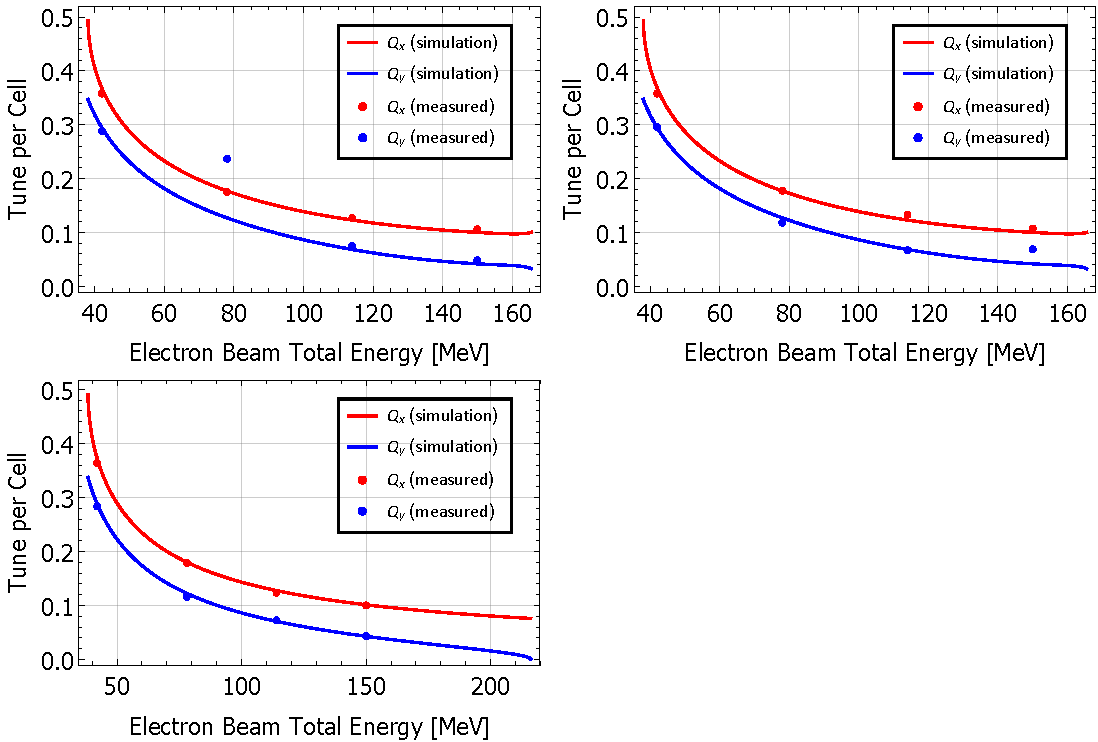
\includegraphics[width=\textwidth]{Figures/CBETA_Multi-Pass_Commissioning/chromaticity/FAFBZX_nominal_tunes.pdf}
\caption{CBETA virtual machine fieldmap tracking simulation derived tunes per cell as a function of electron beam total energy. Measured tunes per cell at the nominal turn energies are also displayed. Top Left: FA arc tune per cell in each transverse plane. Top Right: ZX straight tune per cell in each plane. Bottom Left: FB arc tune per cell in each transverse plane. }
\label{fig:fieldmap_chromaticity_tune}
\end{figure}

Overall the measured nominal tunes show good agreement with the simulations. However, there are some anomalous points such as the 78~\si{\mega\electronvolt} FA arc $Q_{y}$ tune and the 150~\si{\mega\electronvolt} FB arc $Q_{y}$ tune. The cause of these discrepancies is though to be the jitter of the accelerator or incorrect tuning of the accelerator optics within those turns.

Upon further inspection of the tune data, where the energy of the electron bunch is varied by up to 0.5\%, it is noted that this energy variation has distorted the orbit of the final 150~\si{\mega\electronvolt} 4th turn by an intolerable amount as evidenced by Fig.~\ref{fig:FAFBZX_150_tunes}. The optics in this turn are too sensitive to allow for measurement of the chromaticity in the current configuration.

\begin{figure}[!h]
\centering
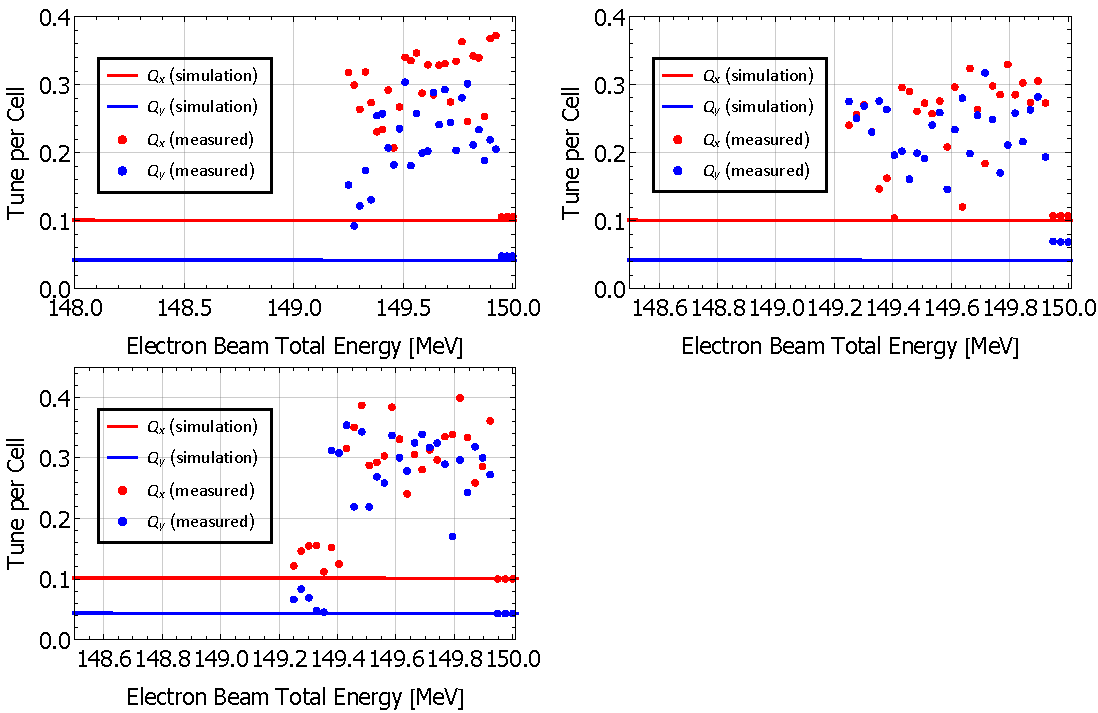
\includegraphics[width=\textwidth]{Figures/CBETA_Multi-Pass_Commissioning/chromaticity/FAFBZX_150_tunes.pdf}
\caption{FFA tune measured data in both $x$ (red point) and $y$ (blue point) against electron bunch energy varied by 0.5\% for the 150~\si{\mega\electronvolt} 4th turn of CBETA in comparison with predicted tune data in the $x$ (red line) and $y$ (blue line) planes from the CBETA virtual machine study. Top Left: FA arc section. Top Right: FB arc section. Bottom Left: ZX straight section.}
\label{fig:FAFBZX_150_tunes}
\end{figure}

Beyond the first 3 measurements closest to the nominal 150~\si{\mega\electronvolt} energy, it is clear in every case that the measured data is erroneous and incomparable with the predictions. On this basis, the 150~\si{\mega\electronvolt} data contradicts the predicted tunes for each of the FFA sections (FA, FB, ZX) and is subsequently discarded from further analysis.

Measurements are further analysed by disregarding any points which are greater than two standard deviations ($2\sigma$) from the mean of the data set. These points are considered anomalous, and by inspection the points labelled anomalous greatly differ from the measured data. These data points may be anomalous due to energy jitter of the linac or peculiarities within the optics configuration used at the time of the measurement. \textcolor{blue}{Needs more work}

The tunes in each plane as a function of electron bunch energy for each of the three remaining turns are presented for the sections of the FFA this measurement has focused upon: FA (Fig.~\ref{fig:FA_analysed_tunes}), FB (Fig.~\ref{fig:FB_analysed_tunes}) and ZX (Fig.~\ref{fig:ZX_analysed_tunes}).

\begin{figure}[!h]
\centering
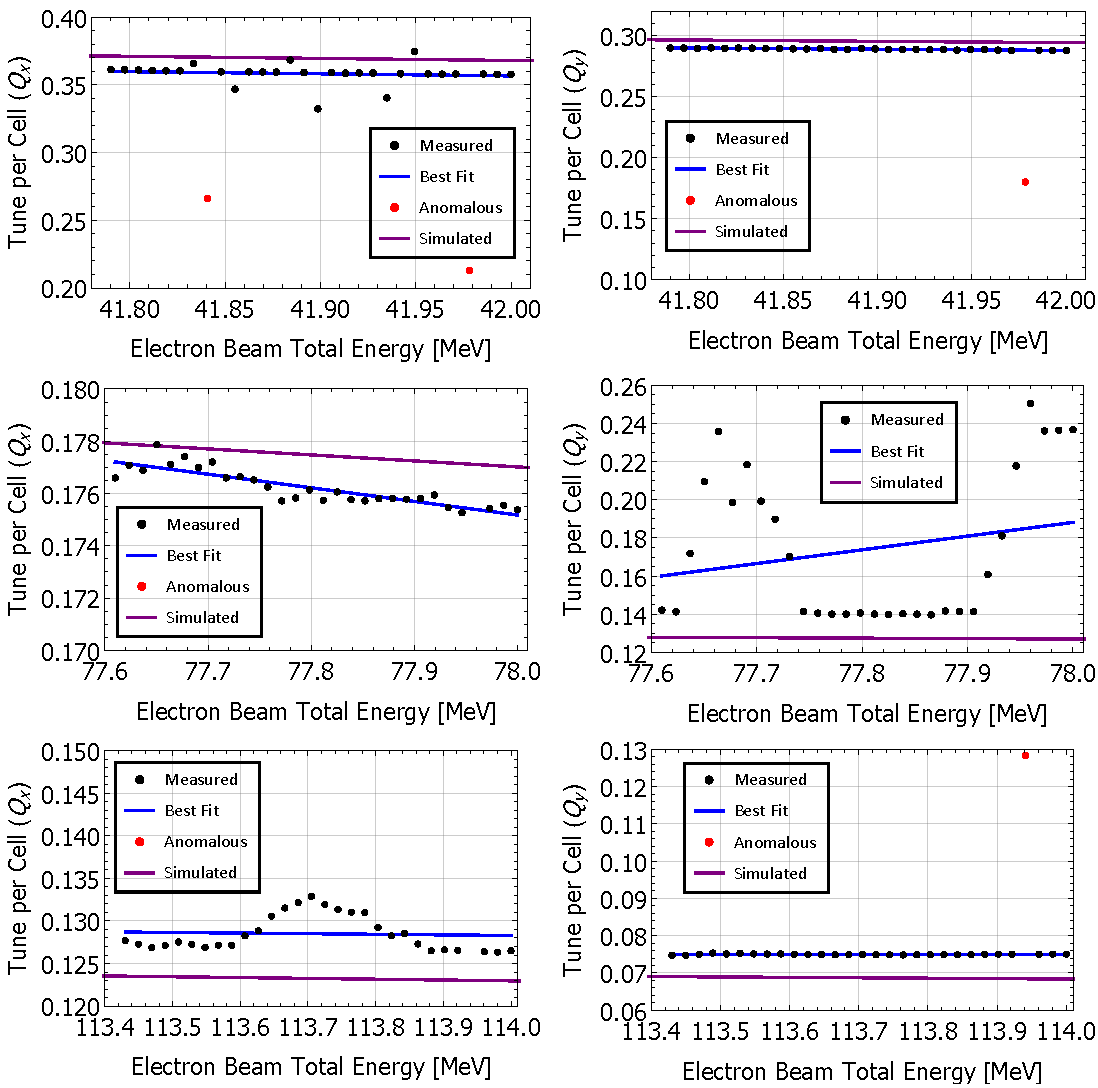
\includegraphics[width=\textwidth]{Figures/CBETA_Multi-Pass_Commissioning/chromaticity/FA_analysed_3turn_tunes.pdf}
\caption{Tunes per cell as a function of electron beam energy for the FA arc. The measured data (black), with a linear regression line of best fit (blue), is shown against the tracking simulation prediction (purple). Data points classified as anomalous (red) are highlighted, these lay further than $2\sigma$ from the mean of the data set. Top Left: 42~\si{\mega\electronvolt} 1st turn tune measurement in the $x$ plane. Top Right: 42~\si{\mega\electronvolt} 1st turn tune measurement in the $y$ plane. Middle Left: 78~\si{\mega\electronvolt} 2nd turn tune measurement in the $x$ plane. Note: a single anomalous point lays outside of the plot range. Middle Right: 78~\si{\mega\electronvolt} 2nd turn tune measurement in the $y$ plane. Bottom Left:  114~\si{\mega\electronvolt} 3rd turn tune measurement in the $x$ plane. Note: a single anomalous point lays outside of the plot range. Bottom Right: 114~\si{\mega\electronvolt} 3rd turn tune measurement in the $y$ plane.}
\label{fig:FA_analysed_tunes}
\end{figure}

\begin{figure}[!h]
\centering
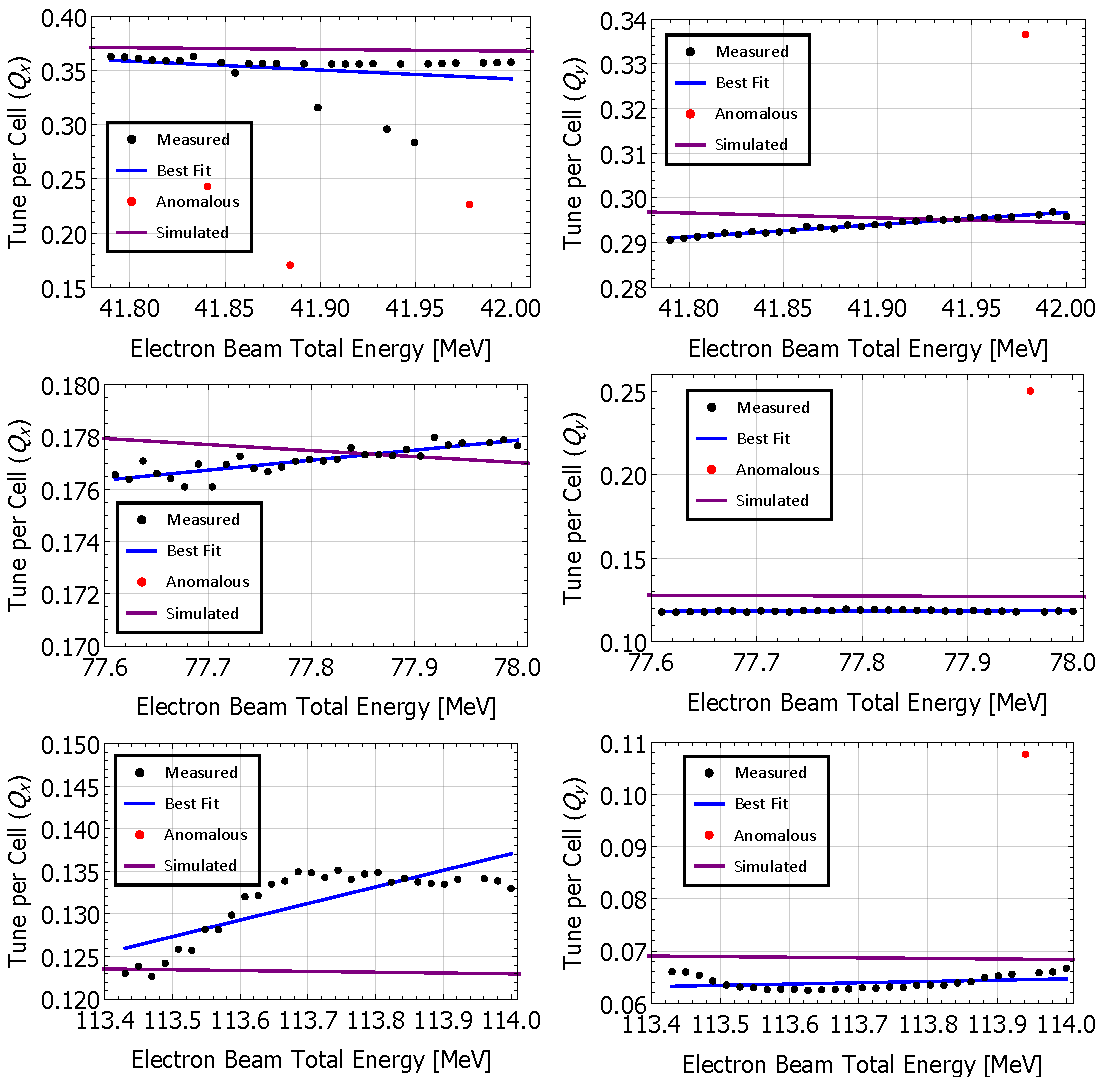
\includegraphics[width=\textwidth]{Figures/CBETA_Multi-Pass_Commissioning/chromaticity/FB_analysed_3turn_tunes.pdf}
\caption{Tunes per cell as a function of electron beam energy for the FB arc. The measured data (black), with a linear regression line of best fit (blue), is shown against the tracking simulation prediction (purple). Data points classified as anomalous (red) are highlighted, these lay further than $2\sigma$ from the mean of the data set. Top Left: 42~\si{\mega\electronvolt} 1st turn measurement in the $x$ plane. Top Right: 42~\si{\mega\electronvolt} 1st turn measurement in the $y$ plane. Middle Left: 78~\si{\mega\electronvolt} 2nd turn measurement in the $x$ plane. Note: a single anomalous point lays outside of the plot range. Middle Right: 78~\si{\mega\electronvolt} 2nd turn measurement in the $y$ plane. Bottom Left: 114~\si{\mega\electronvolt} 3rd turn measurement in the $x$ plane. Note: a single anomalous point lays outside of the plot range. Bottom Right: 114~\si{\mega\electronvolt} 3rd turn measurement in the $y$ plane.}
\label{fig:FB_analysed_tunes}
\end{figure}

\begin{figure}[!h]
\centering
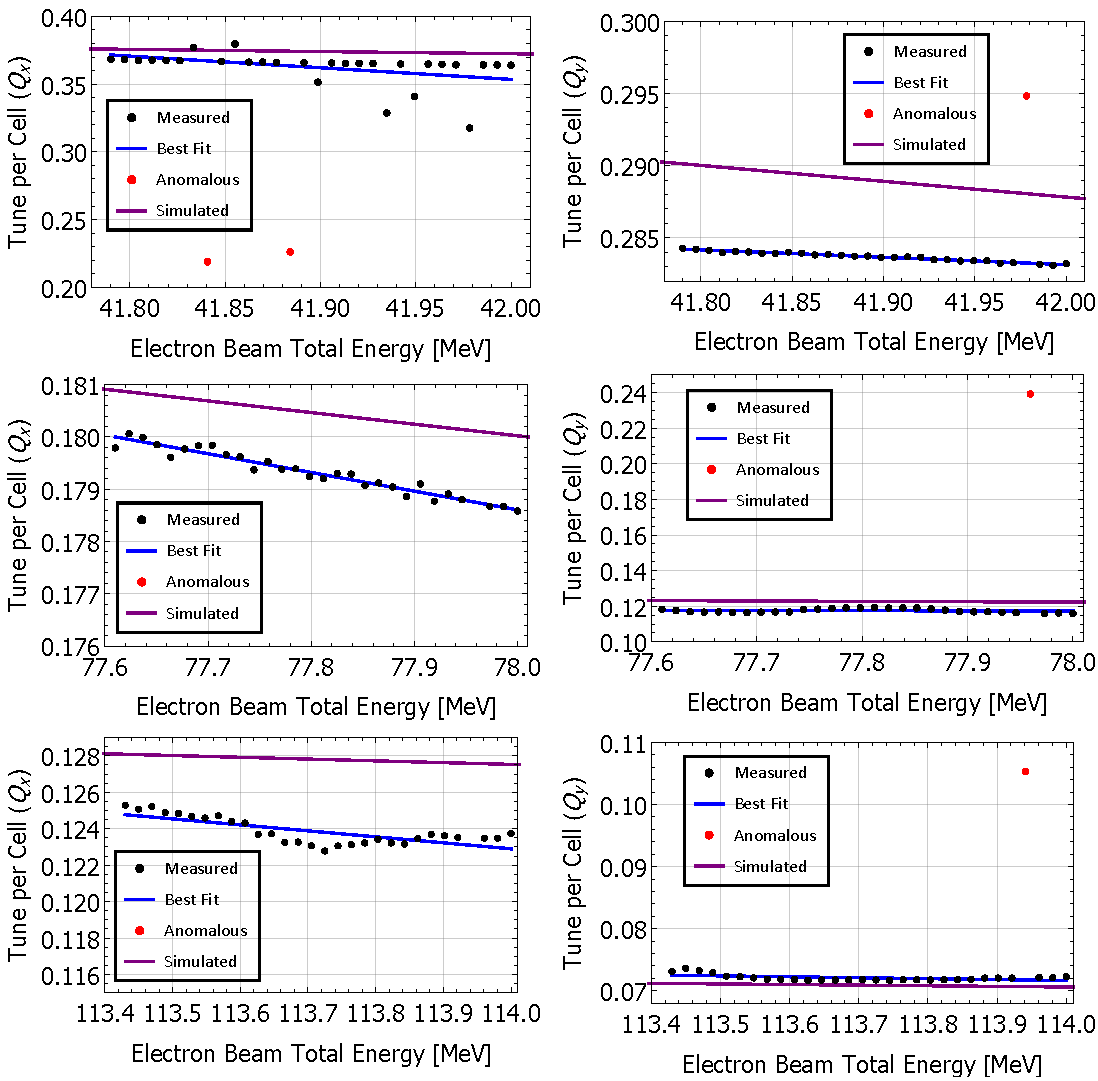
\includegraphics[width=\textwidth]{Figures/CBETA_Multi-Pass_Commissioning/chromaticity/ZX_analysed_3turn_tunes.pdf}
\caption{Tunes per cell as a function of electron beam energy for the ZX straight. The measured data (black), with a linear regression line of best fit (blue), is shown against the tracking simulation prediction (purple). Data points classified as anomalous (red) are highlighted, these lay further than $2\sigma$ from the mean of the data set. Top Left: 42~\si{\mega\electronvolt} 1st turn measurement in the $x$ plane. Top Right: 42~\si{\mega\electronvolt} 1st turn measurement in the $y$ plane. Middle Left: 78~\si{\mega\electronvolt} 2nd turn measurement in the $x$ plane. Note: a single anomalous point lays outside of the plot range. Middle Right: 78~\si{\mega\electronvolt} 2nd turn measurement in the $y$ plane. Bottom Left: 114~\si{\mega\electronvolt} 3rd turn measurement in the $x$ plane. Note: a single anomalous point lays outside of the plot range. Bottom Right: 114~\si{\mega\electronvolt} 3rd turn measurement in the $y$ plane.}
\label{fig:ZX_analysed_tunes}
\end{figure}

\textcolor{blue}{**TALK ABOUT THE TUNE PLOTS**}

The difference in tune per cell from the tune per cell of the nominal energy is then plotted against the fractional variation in electron bunch total energy compared to the nominal energy. Again, the $2\sigma$ statistical test is applied to categorise any points laying outside of $2\sigma$ as anomalous. A line of best fit is plotted using linear regression of the remaining data points. The gradient of the line of best fit on the plot of $\Delta Q$ as a function of $\Delta E_{e}/E_{e}$ is the chromaticity, as per (Eq.~\ref{eq:chromaticity_measurement_central}). Fig.~\ref{fig:FA_dQdEe}, \ref{fig:FB_dQdEe}, \ref{fig:ZX_dQdEe} present the plots of the tune variation as a function of the fractional electron bunch energy variation for each of the three nominal energy cases (42, 78, 114~\si{\mega\electronvolt}) in each plane ($x$ and $y$).    

\begin{figure}[!h]
\centering
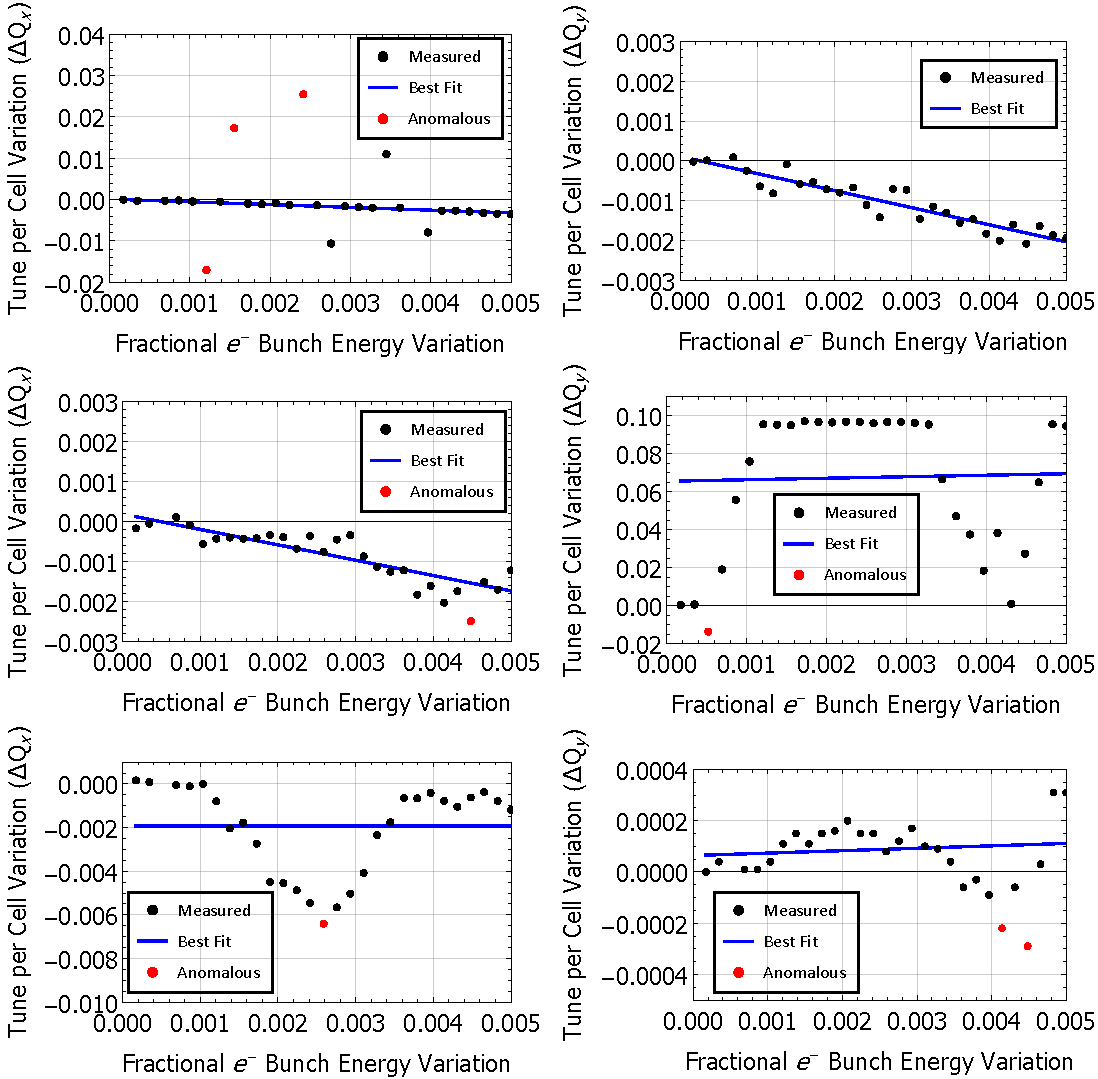
\includegraphics[width=\textwidth]{Figures/CBETA_Multi-Pass_Commissioning/chromaticity/FA_analysed_3turn_dQdEe.pdf}
\caption{Variation in tune per cell from the nominal energy tune per cell as a function of the fractional variation in electron bunch energy from the nominal energy for the FA arc. The measured data (black) is plotted with a linear regression line of best fit (blue), with anomalous points (red) highlighted. Top Left: 42~\si{\mega\electronvolt} 1st turn measurement in the $x$ plane. Top Right: 42~\si{\mega\electronvolt} 1st turn measurement in the $y$ plane. Middle Left: 78~\si{\mega\electronvolt} 2nd turn measurement in the $x$ plane. Middle Right: 78~\si{\mega\electronvolt} 2nd turn measurement in the $y$ plane. Bottom Left: 114~\si{\mega\electronvolt} 3rd turn measurement in the $x$ plane. Bottom Right: 114~\si{\mega\electronvolt} 3rd turn measurement in the $y$ plane.}
\label{fig:FA_dQdEe}
\end{figure}

\begin{figure}[!h]
\centering
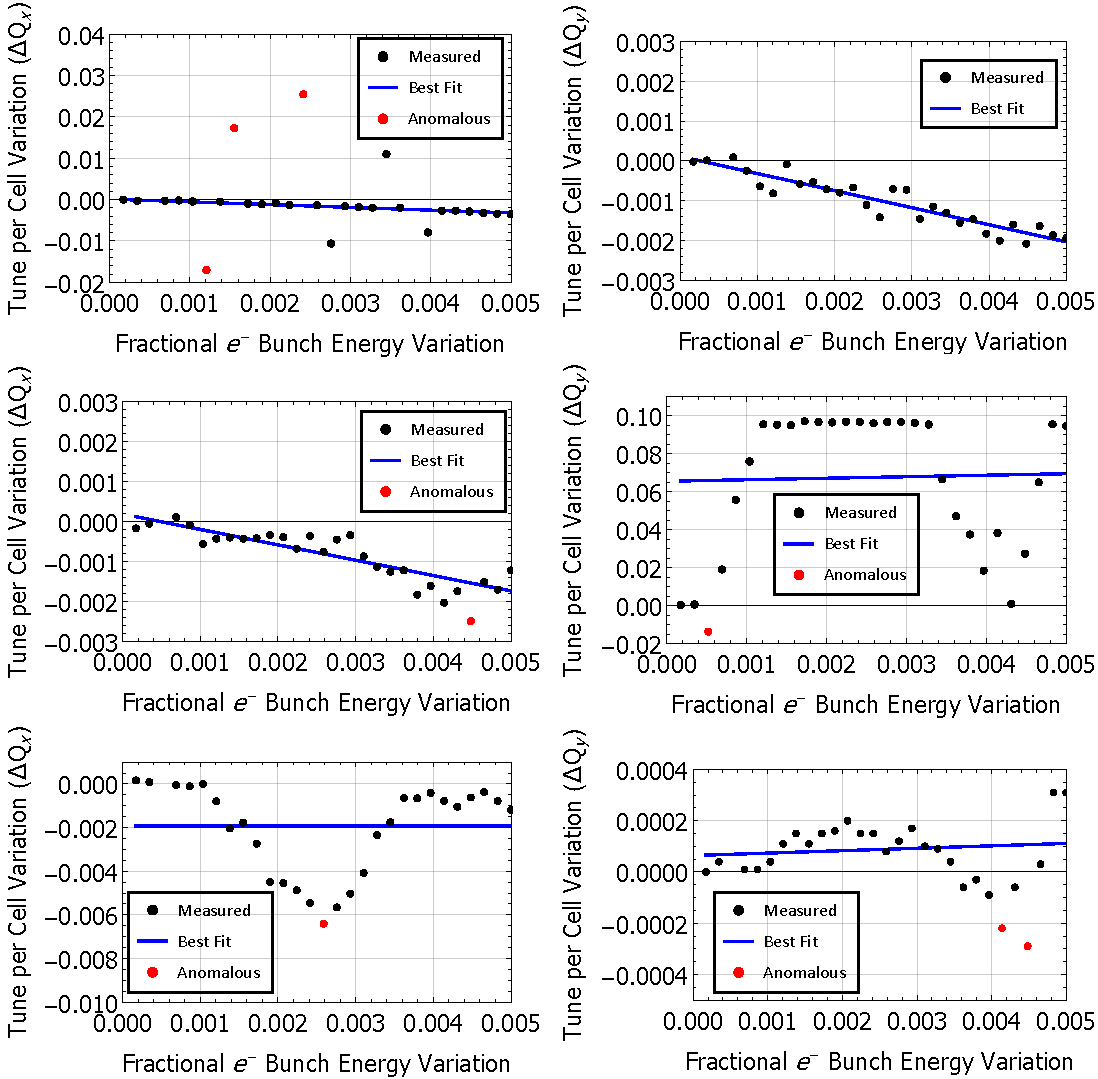
\includegraphics[width=\textwidth]{Figures/CBETA_Multi-Pass_Commissioning/chromaticity/FB_analysed_3turn_dQdEe.pdf}
\caption{Variation in tune per cell from the nominal energy tune per cell as a function of the fractional variation in electron bunch energy from the nominal energy for the FB arc. The measured data (black) is plotted with a linear regression line of best fit (blue), with anomalous points (red) highlighted. Top Left: 42~\si{\mega\electronvolt} 1st turn measurement in the $x$ plane. Note: two anomalous points in this data set lay outside of the plotting range. Top Right: 42~\si{\mega\electronvolt} 1st turn measurement in the $y$ plane. Middle Left: 78~\si{\mega\electronvolt} 2nd turn measurement in the $x$ plane. Middle Right: 78~\si{\mega\electronvolt} 2nd turn measurement in the $y$ plane. Bottom Left: 114~\si{\mega\electronvolt} 3rd turn measurement in the $x$ plane. Bottom Right: 114~\si{\mega\electronvolt} 3rd turn measurement in the $y$ plane.}
\label{fig:FB_dQdEe}
\end{figure}

\begin{figure}[!h]
\centering
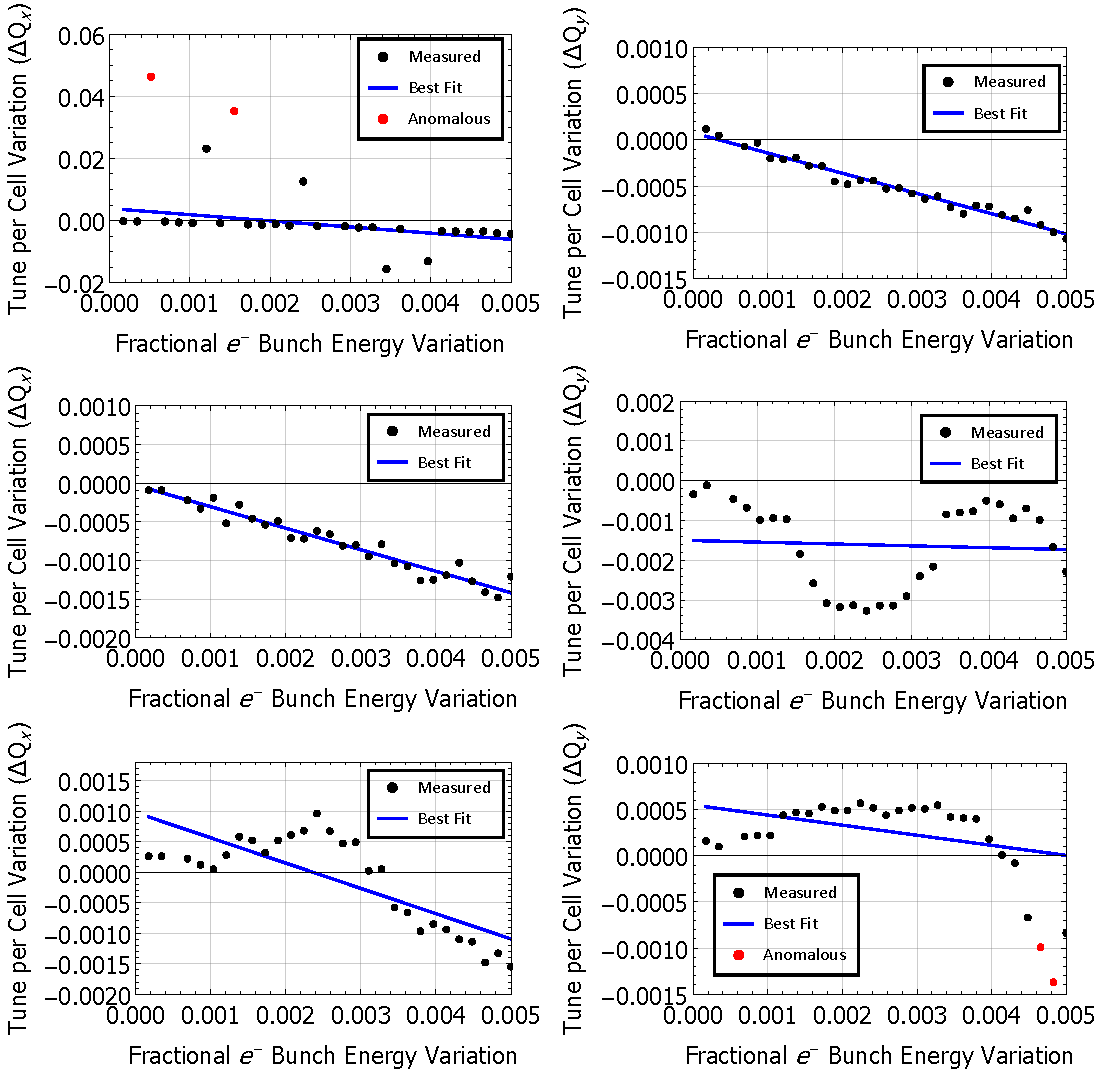
\includegraphics[width=\textwidth]{Figures/CBETA_Multi-Pass_Commissioning/chromaticity/ZX_analysed_3turn_dQdEe.pdf}
\caption{Variation in tune per cell from the nominal energy tune per cell as a function of the fractional variation in electron bunch energy from the nominal energy for the ZX straight. The measured data (black) is plotted with a linear regression line of best fit (blue), with anomalous points (red) highlighted. Top Left: 42~\si{\mega\electronvolt} 1st turn measurement in the $x$ plane. Top Right: 42~\si{\mega\electronvolt} 1st turn measurement in the $y$ plane. Middle Left: 78~\si{\mega\electronvolt} 2nd turn measurement in the $x$ plane. Middle Right: 78~\si{\mega\electronvolt} 2nd turn measurement in the $y$ plane. Bottom Left: 114~\si{\mega\electronvolt} 3rd turn measurement in the $x$ plane. Bottom Right: 114~\si{\mega\electronvolt} 3rd turn measurement in the $y$ plane.}
\label{fig:ZX_dQdEe}
\end{figure}

\textcolor{blue}{**TALK ABOUT THE dQdE PLOTS**}

The chromaticity has been calculated in each plane for each of the three nominal energies using the line of best fit in each plot in Fig.~\ref{fig:FA_dQdEe}, \ref{fig:FB_dQdEe}, \ref{fig:ZX_dQdEe} and these are tabulated in Table~\ref{tab:FAFBZX_measured_chromaticity}. \textcolor{blue}{**TALK ABOUT THE MEASUREMENTS**} 

\begin{table}[!h]
\centering
\caption{chromaticity measured data}
\begin{tabular}{lcccccc}
\hline\hline
FFA Section & \multicolumn{2}{c}{FA} & \multicolumn{2}{c}{FB} & \multicolumn{2}{c}{ZX} \\
\hline
Nominal Electron Energy (\si{\mega\electronvolt}) & $Q'_{x}$ & $Q'_{y}$ & $Q'_{x}$ & $Q'_{y}$ & $Q'_{x}$ & $Q'_{y}$ \\
\hline
42 & -0.669 & -0.429 & -1.22 & 1.19 & -1.99 & -0.219 \\
78 & -0.384 & 0.793 & 0.308 & 0.0768 & -0.278 & -0.0468 \\
114 & 5.93$\times 10^{-4}$ & 9.47$\times 10^{-3}$ & 2.26 & 0.187 & -0.414 & -0.109 \\ 
\hline\hline
\end{tabular}
\label{tab:FAFBZX_measured_chromaticity}
\end{table}

The measured chromaticities are plotted against the predicted chromaticity which is calculated via the derivative of the virtual machine tune--electron bunch energy for each plane and each of the three nominal energies in Fig.~\ref{fig:FAFBZX_chromaticity}. 

\begin{figure}[!h]
\centering
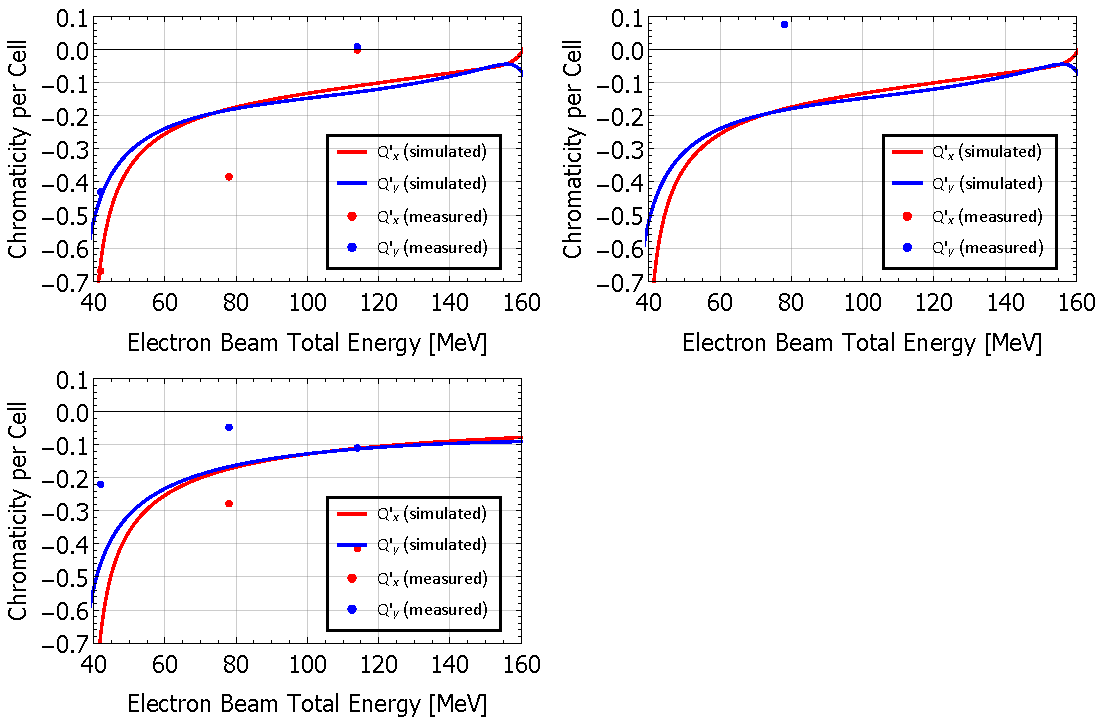
\includegraphics[width=\textwidth]{Figures/CBETA_Multi-Pass_Commissioning/chromaticity/FAFBZX_chromaticity.pdf}
\caption{Plots of the measured chromaticity in the $x$ (red point) and $y$ (blue point) planes, for the first three nominal energies, against the chromaticity predicted via simulation using the CBETA virtual machine in the $x$ (red line) and $y$ (blue line) planes. Top Left: Chromaticity measurement and simulation prediction in both planes through the FA arc. Note: the measured 78~\si{\mega\electronvolt} $Q'_{y}$ point lays outside of the plot range. Top Right: Chromaticity measurement and simulation prediction in both planes in the FB arc. Note: all measured points except the 78~\si{\mega\electronvolt} $Q'_{y}$ point lay outside of the plot range. Bottom Left: Chromaticity measurement and simulation prediction in both planes in the ZX straight. Note: the measured 42~\si{\mega\electronvolt} $Q'_{x}$ point lays outside of the plot range.}
\label{fig:FAFBZX_chromaticity}
\end{figure}

The predictions in Fig.~\ref{fig:FAFBZX_chromaticity} show that the chromaticity of each of the sections of the CBETA FFA is expected to be negative throughout the whole energy range of the CBETA operation however, as seen in Table~\ref{tab:FAFBZX_measured_chromaticity}, some measurements show large positive chromaticities such as the 114~\si{\mega\electronvolt} FB arc $Q'_{x} = 2.26$ measurement. Good agreement with the simulated chromaticity is achieved in several measurements for example the 42~\si{\mega\electronvolt} FA arc chromaticities in each plane.   

\subsection{Discussion}
\label{sec:chromaticity_discussion}

Unfortunately, this script was only tested on the last day of operation in the CBETA multi-pass commissioning period. Due to energy drift and jitter in the linac, many tune measurements appear to be distorted. With more data collection on a series of runs the effect of energy drift and linac jitter could be excluded from the data set which could improve the quality of the chromaticity measurement.

The general consistency of the nominal tunes with virtual machine predictions in Fig.~\ref{fig:fieldmap_chromaticity_tune} and the general consistency of the measured and predicted tune per cell variation with electron beam energy in Fig.~\ref{fig:FA_analysed_tunes}, \ref{fig:FB_analysed_tunes}, \ref{fig:ZX_analysed_tunes}, as well as the agreement demonstrated the multi-pass CBETA paper \cite{bartnik2020cbeta}, gives confidence that the existing method of measuring tune is accurate. However, the chromaticity measurement appears to be more sensitive to small changes in energy and measured BPM position. \textcolor{blue}{**I DON'T REALLY KNOW WHAT TO SAY**} 

\end{document}